\documentclass[twocolumn]{article}
\usepackage[spanish]{babel}
\usepackage{caption}
\usepackage{graphicx}
\usepackage{amsmath}
\setlength{\parindent}{0pt}

\author{Josué Villasante}
\title{Patrón de interferencia}

\begin{document}
	\maketitle

	\section{Objetivo}
		Crear un patrón de interferencia producido por la división y posterior unión de un mismo haz de luz de un láser.

	\section{Procedimiento}
		El láser utilizado tuvo una potencia menor a 20mW y una longitud de onda de 633nm.

		Primero se empezó alineando el haz de luz luego de los dos primeros espejos, sobre la línea de orificios en la mesa. Luego se colocó la lamina retardadora y el PBS (polarizing beam splitter) lo más cercano al segundo espejo, e igualmente se intentó alinear el haz del láser polarizado horizontalmente de manera paralela a los orificios de la mesa. Rápidamente, se observó que no se podía alinear este haz sin evitar que parte del reflejo del PBS regrese al láser produciendo un haz distorsionado.

		\begin{center}
			\includegraphics[width=100pt]{img/layout_attempt.pdf}
			\captionof{figure}{Arreglo de primera configuración.}
		\end{center}

		Por lo tanto, para evitar esto se colocó la lamina retardadora y el PBS a una mayor distancia del segundo espejo, y, por otro lado, se colocó un iris inmediatamente luego del láser. La mayor distancia permitió que el desvío de la reflexión sea mayor. El iris se utilizó para bloquear este haz de luz reflejado de regreso por el PBS.

		Se continuó colocando el espejo 3 y 4, e igualmente se alineó ambos haces con los orificios de la mesa. Luego se colocó el BS (beam splitter) y se lo alineó de tal forma que produzca un solo punto en ambos lados. Hasta ese momento no se observó ningún patrón de interferencia.

		\begin{center}
			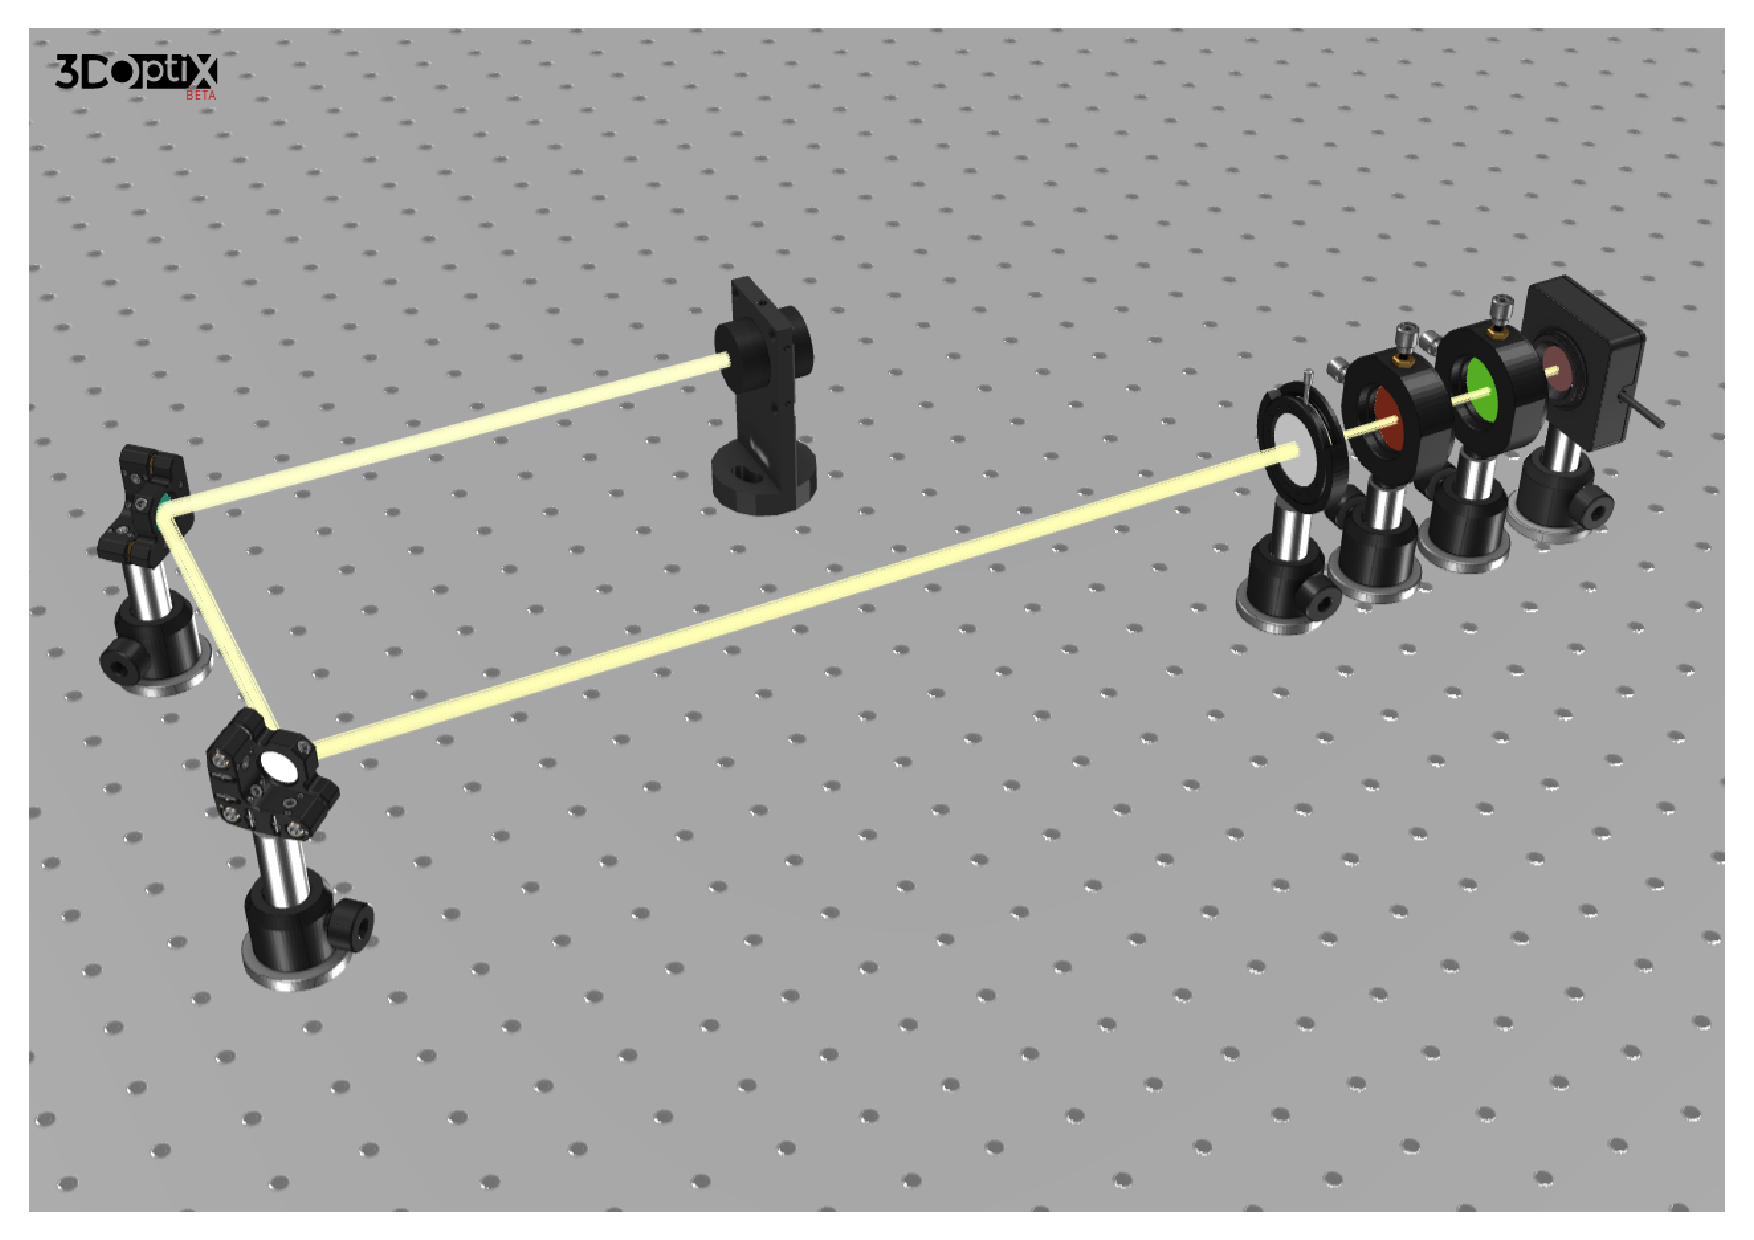
\includegraphics[width=150pt]{img/layout.pdf}
			\captionof{figure}{Arreglo final del experimento.}
			\label{final_layout}
		\end{center}

		Para observar el patrón era necesario colocar un polarizador a 45$^{\circ}$. Para esto, se colocó temporalmente el polarizador entre el espejo 3 y el PBS, y se lo rotó hasta encontrar la posición con menor potencia (sin mover el indicador de ángulo). La menor potencia encontrada fue alrededor de 5$\mu W$. Posteriormente, usando las marcas de ángulos del polarizador, se lo rotó hasta marcar 45$^{\circ}$. Con el polarizador listo, se lo movió a su posición final en la mesa tal cómo se ve en la figura \ref{final_layout}.

		A partir de este momento se ya pudo observar el patrón de interferencia. Para agrandar el punto resultante se colocó un lente convergente, y se pudo ver claramente el patrón.

	\section{Resultados}
		El patrón de interferencia observado fue el siguiente.

		\begin{center}
			\includegraphics[width=100pt]{img/interference.png}
			\captionof{figure}{Patrón de interferencia observado.}
			\label{interference}
		\end{center}

	\section{Discusión}
		El alineamiento y superposición no es perfecto, y esto es lo que produce el patrón. Tal cómo se puede observar en la figura \ref{alignment}, es la rotación del BS que permite suponer los dos haces de luz en un mismo punto.

		\begin{center}
			\includegraphics[width=100pt]{img/alignment.pdf}
			\captionof{figure}{Exageración de la imperfección en el alineamiento en el BS. Los colores solo permiten diferenciar los dos haces.}
			\label{alignment}
		\end{center}

		El pequeño ángulo que forman estos dos haces finales es el que permite que los frentes de onda se interfieran de manera constructiva o destructiva. Esto se observa si vemos de cerca ambos frentes de onda en el lugar dónde impactan al final.

		\begin{center}
			\includegraphics[width=200pt]{img/zoom_in.png}
			\captionof{figure}{Acercamiento a los dos frentes de onda en el lugar de impacto.}
			\label{zoom_in}
		\end{center}

		En la imagen tenemos el haz azul y el rojo. Donde se ve un solo color tendríamos interferencia destructiva, y dónde se ve blanco o un ligero morado tendríamos interferencia constructiva. De esta manera los colores nos permiten visualizar la manera en que la interferencia se produce.

		Por otro lado, vemos que el tamaño del haz azul es más grande debido al ángulo por el cual es reflejado por el BS. En la parte de la izquierda dónde no hay superposición no habría interferencia.

		Por último, para que se produzca la mayor cantidad de interferencia es necesario que ambos haces tengan la misma polarización. Antes de pasar por el polarizador se tiene superpuesto un haz polarizado verticalmente y otro horizontalmente. Por estos motivos es necesario colocar el polarizador al final del arreglo, convirtiendo la polarización de ambos haces a 45$^{\circ}$.
\end{document}